\chapter{High Level Design Description}
\label{high_level}
This chapter gives an overview of the high level design. It includes a functional block diagram of the system, which partitions the design of the system into blocks, and depicts the interactions between the blocks. Furthermore it gives an overview of the system states through a state machine diagram. 

\subsection{Functional block diagram}
The functional block diagram is shown in figure \ref{fig:func_block_diagram}:

\begin{figure}[H]
\centering
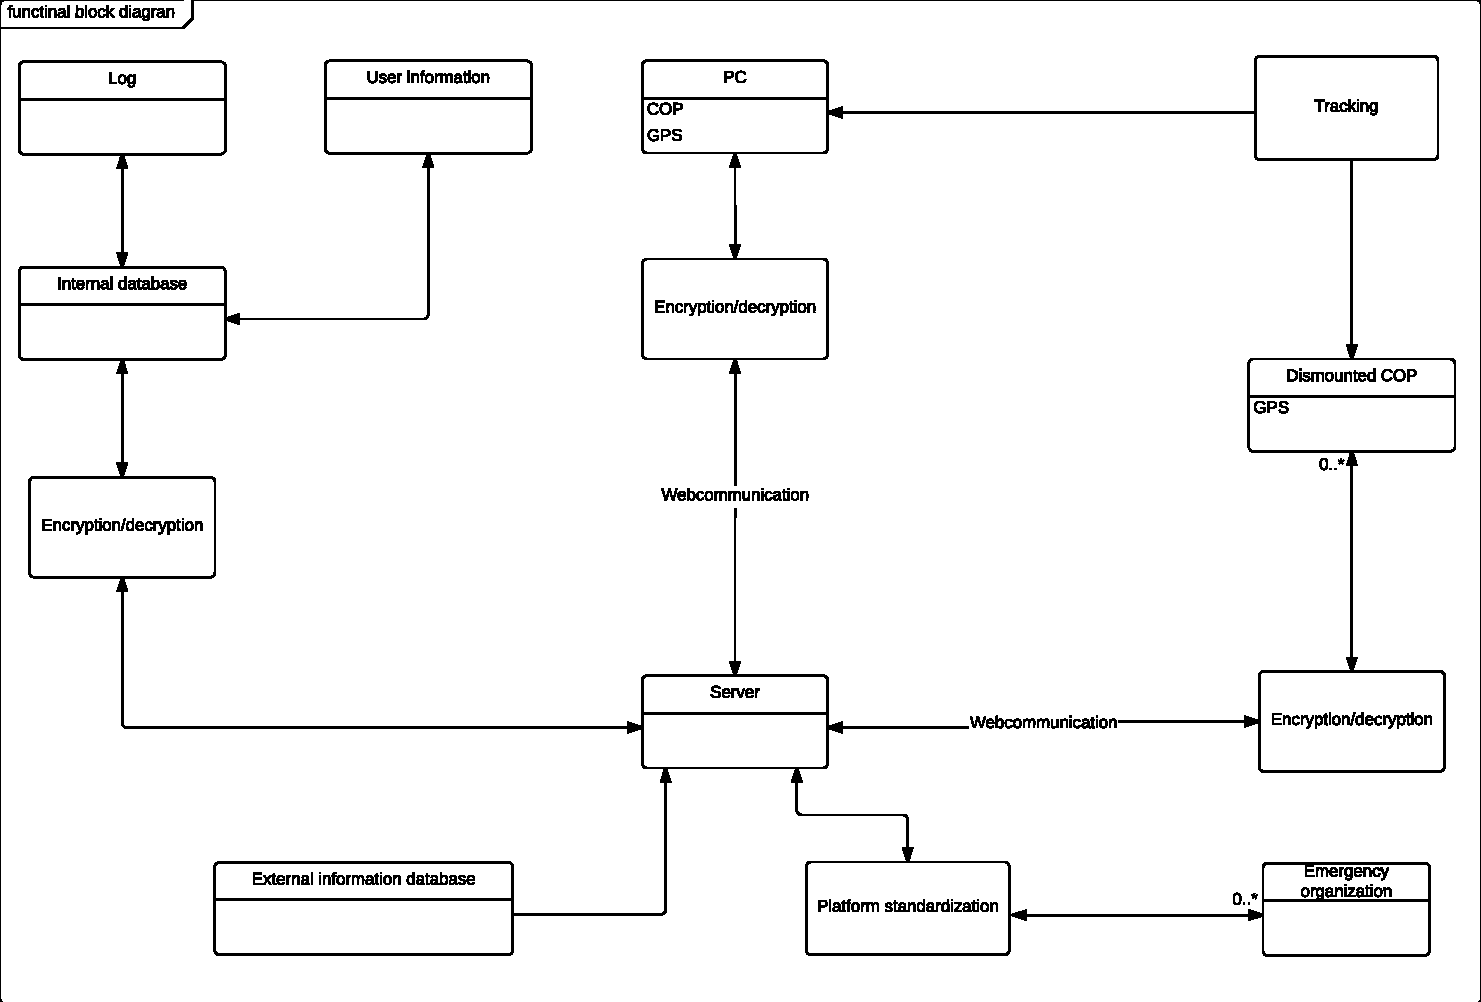
\includegraphics[width=0.95\textwidth]
{billeder/functional_block_diagram.pdf}
\caption{Functional block diagram of the system.}
\label{fig:func_block_diagram}
\end{figure}

The diagram consists of system-blocks and function-blocks. The system-blocks are depicted as two-compartment blocks with the name of the block in the first compartment, and sub parts in the second compartment. The functions are blocks with a single compartment, containing the name of the function. The system-blocks are actual parts of the system, while the function-blocks are functions and actions that are carried out in the system. The data flow between the blocks are depicted with arrows, whose direction dictates the direction of the data flow. 

\subsubsection{Block description}
In this section a short description of each system- and function-block is given.

\textbf{System-blocks}
\begin{enumerate}
\item[•] \textbf{PC:} This block constitutes the machine in the head quarter (HQ) on which the COP-software will be executed. It also has a GPS module, so that the location of the HQ is always known. The PC is to be connected to the internet, in order to be able to communicate with the rest of the system.
\item[•] \textbf{Server:} The server will facilitate communication between the other blocks. In addition, it will store user information along with logs locally in an internal database.
\item[•] \textbf{Log:} The log will contain log entries with information about previous events.
\item[•] \textbf{User information:} This block will contain information about the users of the system.
\item[•] \textbf{Internal database:} The internal database will be responsible for storing the log and user information.
\item[•] \textbf{External information database:} This block constitutes the source of static and dynamic information, that the COP will make available to the user.
\item[•] \textbf{Dismounted COP:} This block constitutes the machine on which the condensed COP-software will be executed. The dismounted COP will be used by the dismounted users in the field. It has a GPS module, so that the location of the dismounted users is always known. Furthermore it has a GSM module so that it will be able to communicate with the rest of the system.
\item[•] \textbf{Emergency organization:} These blocks constitute the platforms currently employed by the various emergency organizations using the system.
\end{enumerate}


\textbf{Function-blocks}
\begin{enumerate}
\item[•] \textbf{Encryption/decryption:} These blocks will be responsible for encrypting outgoing data and decrypting incoming data in the communication between the various system blocks.
\item[•] \textbf{Tracking:} This block constitutes all communication with GPS-satellites.
\item[•] \textbf{Platform standardization:} This block is responsible for unifying all communication between the various emergency organizations using the system, and the COP/dismounted COP.
\end{enumerate}

\subsection{State machine diagram}
The the state machine diagram is shown in figure \ref{fig:state_diagram}:

\begin{figure}[H]
\centering
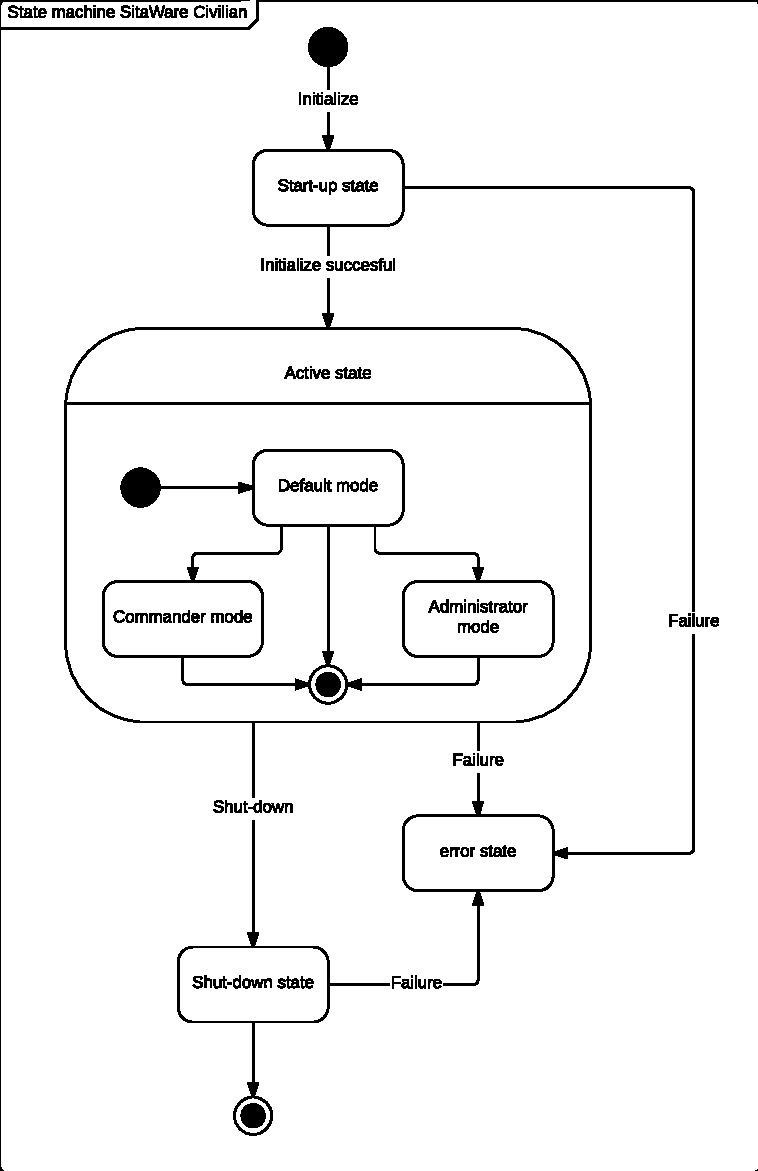
\includegraphics[width=0.95\textwidth]
{billeder/state_machine_pdd.pdf}
\caption{State machine diagram of the system.}
\label{fig:state_diagram}
\end{figure}

In accordance with the System Requirement Specification, the system has four states: a start-up state, an active state, an error-state and a shut-down state. When in the active state, the system can operate in three different modes. If an error occurs anywhere in the start-up, active or shut-down state, the system will enter an error state, where the error can be remedied.